\section{Candidate Graphs to Unique Useful Graphs}

In the previous section an approach for enumerating architectures based on the consideration of every potential \mypm{} was outlined. However, there are a number of deficiencies in this set of architectures, including infeasible graphs based on practical constraints for a specific architecture design problem, and repeated graphs in the modeling sense. The following two subsections address architecture feasibility and uniqueness, respectively.

\subsection{Network Structure Constraints\label{sec:ch2:NSC}}

We define feasibility as a candidate architecture's satisfaction of all \glsfirstplural{NSC} for a particular architecture design problem. Similar to the rules in generative design approaches, the creation of the set of network structure constraints for a particular architecture design problem is subject to the creativity and intuition of the designer. Some of these constraints may be fairly self-evident while others might be vague or contentious (Ref.~\cite{Wyatt2012a} discusses these issues). Wyatt et al. describe four types of NSCs that are sufficient to define almost all aspects of realizability of an architecture and are summarized briefly (without edge coloring considerations) as \cite{Wyatt2012a}:
\begin{enumerate}[label=$\bullet$, widest=$\bullet$, nosep]
\item \Glsfirstplural{CNC} prescribe how many components of a given type must be present
\item \Glsfirstplural{DCC} prescribe which component types may be connected together by which connection types and cardinality of the connections
\item \Glsfirstplural{FOC} prescribe how many connections that components of a certain type must have in total
\item \Glsfirstplural{ICC} prescribe how many continuous paths there must be from every component of one type to every component of another type
\end{enumerate}

Graph generating algorithms designed to always satisfy certain NSCs could be more useful since all of the generated graphs would be feasible with respect to those certain NSCs.
Furthermore, graph generating algorithms can also be designed to produce graphs that have a higher proportion that satisfies certain NSCs than more naive approaches.
Some of the NCSs that are not satisfied can be with edits to the graph.
The only operation that will be considered here is the removal of vertices $G^{CC}$ and the corresponding edges and labels as it will maintain certain properties of the graph structure space $\mathcal{G}_1$.
Other operations such as vertex insertion, edge insertion, or label substitution destroy the analysis of the design space coverage that is possible with an enumerative \mypm{} approach.
Next, several common NSCs (denoted with \gls{S}) are described along with the specifics of checking their satisfaction with available graph analysis tools.

\begin{enumerate}[label=$S_{\!\arabic*}$]

\item \label{ch2:s1} Every graph must be a connected graph (ICC). A graph is termed connected if there is a path from any vertex to any other vertex in the graph \cite[p.~18]{Diestel2000a}. This can be checked with the connectivity matrix, $A_C(G)$, in Eqn.~(\ref{eq:ch2:connectivity}). If all entries in this matrix are not 1, then the graph is not connected.

\item \label{ch2:s2} Every graph can only have a maximum number of a given component type (CNC). This is defined by $R$ in the architecture definition three-tuple so is naturally handled by a \mypm{} approach. An example: `Every suspension must have less than 3 springs'.

\item \label{ch2:s3} Every graph must have a specific number of certain component types (CNC). These mandatory components will be captured with a vector \gls{M} of length $n_C$. The elements of $M$ are binary with a $1$ indicating all replicates of the component type must be present in the graph. An example: `Every hybrid powertrain must have an engine and a vehicle'.

\item \label{ch2:s4} Every graph must have specific component types connected to each other (ICC). This can be checked with the connectivity matrix in Eqn.~(\ref{eq:ch2:connectivity}). If nonzeros are not present at every location where a path must exist between component types, then the graph is infeasible. If we require \ref{ch2:s1} and \ref{ch2:s3}, then we can leverage the vector $M$ in \ref{ch2:s3} to satisfy both constraints by checking $A_C(G)$ such that all mandatory components are connected to each other. An example: `Every hybrid powertrain must have an engine connected to a vehicle'.

\item \label{ch2:s6} Every graph must have vertices whose number of unique edges is within a specific range (FOC). The values in $P$ can define the upper bound for each vertex since components are defined by a certain number of ports. For even port numbered component types the lower bound is 0 and 1 for odd. This can be checked summing row-wise (or column-wise) the symmetric adjacency matrix $A(G)$ and comparing these sums to the appropriate index in $P$. This type of NSC is sometimes termed a degree-constrained subgraph problem \cite[p.~217]{Lawler1976a}. A \mypm{} approach naturally satisfies this constraint. An example: `Every spring must have between 0 and 2 unique edges'.

\item \label{ch2:s7} Every graph must have vertices with a specified number of unique connections (FOC). This is a stronger form of \ref{ch2:s6} where both the upper and lower bound can be determined by $P$ and is sometimes termed a factors problem  \cite[p.~218]{Lawler1976a}. An example: `Every spring must have exactly 2 unique edges'.

\item \label{ch2:s5} Every graph must have edges between vertices that are feasible (DCC). We can specify that certain component types cannot be connected to other component types with a reduced potential adjacency matrix $A_{\gls{reduced}}$. This $n_C \times n_C$ binary matrix will have 1 entries indicating a connection is feasible and 0 entries for infeasible. 
This constraint can be checked by verifying that each 1 in $A(G)$ has a corresponding 1 in the potential adjacency matrix. No self-loops in a specific component type can be enforced with a 0 at the appropriate location on the diagonal of $A_R$. A \mypm{} approach does not satisfy this constraint as all connections between ports are considered feasible.  An example: `Every translational spring cannot be connected to any rotational damper'.

\end{enumerate} 

The ordering of the constraints matters if vertices are to be removed to satisfy certain constraints. The following procedure is assumed:
\begin{enumerate}[nosep]
\setcounter{enumi}{-1}
\item \ref{ch2:s2} and \ref{ch2:s6} naturally satisfied with a \mypm{} approach
\item \label{ch2:step1} Check \ref{ch2:s3} and \ref{ch2:s4} simultaneously using $M$ since they can be checked without needing to remove the removable components
\item \label{ch2:step2} Remove components that don't satisfy \ref{ch2:s3} and \ref{ch2:s4}; thus satisfying \ref{ch2:s1} 
\item Check \ref{ch2:s7} 
\item \label{ch2:step4} Check \ref{ch2:s5}
\item Check any other constraints
\end{enumerate} 

\noindent The specific steps are only performed if the constraint is present in a specific architecture design problem. The ordering of \ref{ch2:s7}, \ref{ch2:s5}, and the other previously undefined constraints could be performed in an alternative order as long as they are checked after removable components are removed. This is so that a candidate architecture is not declared infeasible if only removed components and their connections violate the constraints.

The graph structure space defined as graphs that satisfy the present NSCs and $(C,R,P)$ is denoted $\mathcal{G}_2 \subseteq \mathcal{G}_1$. The NSCs \{\ref{ch2:s1}, \ref{ch2:s3} \ref{ch2:s4}\} are assumed to be all present or none present to simplify the discussion as many common architecture design problems require all three. With the NSCs outlined, a \textit{useful graph} is defined as one that is feasible with respect to the NSCs.

\subsubsection{Comparison to Another Method\label{sec:ch2:comparison}}

At this point, it is imperative to compare the \mypm{} approach to another graph numerical representation scheme that can be used for enumeration: \glsfirstplural{ISB} \cite{Wyatt2014a}. This scheme is far more general than the proposed  \mypm{} approach as it allows for directed graphs, edge coloring, enumeration of potential colored label sets, and variable number of nodes. All permutations of the candidate adjacency matrices are considered. The graph structure space for the ISB approach is denoted $\mathcal{G}_0$ since $\mathcal{G}_1 \subseteq \mathcal{G}_0$. However with this generality comes an enormous space, potentially too large to be useful for certain problems. 

We can analyze this statement by observing how the ISB block method handles some of the proposed NSCs. For a fair discussion, we should restrict the space to a certain block (fixed number of vertices and color label set ordering). Then both \ref{ch2:s2} and \ref{ch2:s5} can be naturally satisfied by removing the infeasible entries in the adjacency matrix. However, \ref{ch2:s6} is not satisfied for large portions of $\mathcal{G}_0$; the degree of a vertex is not directly controlled. Once additional NSCs are added, the probability that an index results in a feasible graph might be so small that none are ever found. 

\indent To illustrate this consider the number of permutations of $A(G^{CC})$ with $N_C$ components \cite{Wyatt2014a}:
\begin{align}
\gls{adjfunc} = 2^{\nicefrac{N_C (N_C - 1)}{2}}
\end{align}

\noindent with the first several values being $\mathcal{T}(1) = 1$, $\mathcal{T}(2) = 2$, $\mathcal{T}(3) = 8$, $\mathcal{T}(4) = 64$, $\mathcal{T}(5) = 1,024$, $\mathcal{T}(6) = 32,768$, $\mathcal{T}(7) = 2,097,152$, $\mathcal{T}(8) = 268,435,456$. Now consider the case when $N_P = 30$ and $N_C = 20$, then there are $6\times 10^{15}$ \mypm{}s versus $2\times 10^{57}$ adjacency matrix permutations. Both numbers are quite large but a clear combinatorial advantage is seen with the \mypm{} approach (see Fig.~\ref{fig:ch2:power2comparison}). This will be exacerbated when structured components considered.  However, since $N_P$ and $N_C$ can be different, there are some combinations where $\mathcal{T}(N_C)$ is actually smaller than $\mathcal{D}(N_P)$. This is shown in the figure with the curved line $\mathcal{D}(N_P) = \mathcal{T}(N_C)$. Most architecture design problems are above this line.

\begin{figure}
\centering
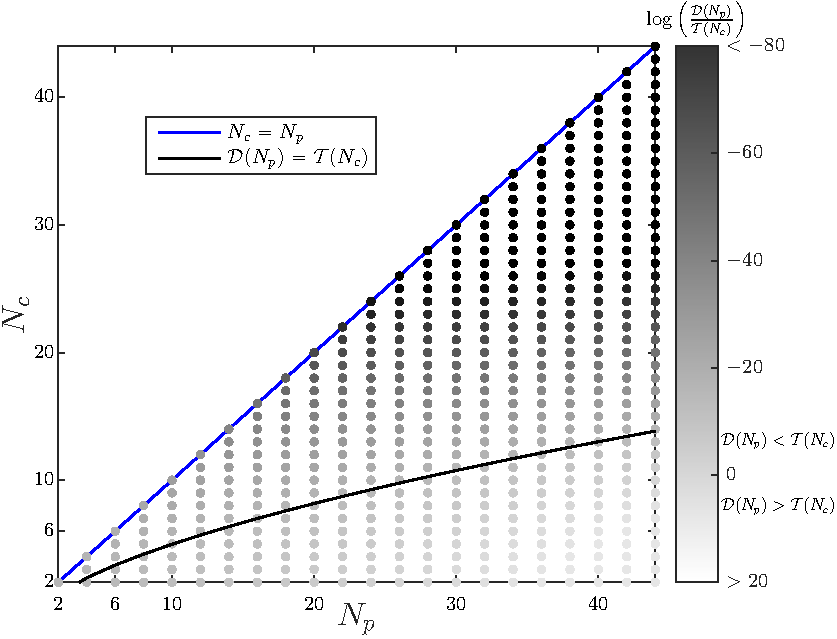
\includegraphics[width=0.6\columnwidth]{../ch2/figures/power2comparison}
\caption[Comparison between a \mypm{} approach and adjacency matrix approach.]{Comparison of number of graphs with \mypm{} approach and adjacency matrix approach.\label{fig:ch2:power2comparison}}
\end{figure}

A \mypm{} approach can be seen as an alternative to permuting all possible adjacency matrices assuming the architecture design problem is based on $(C,R,P)$ with NSC \ref{ch2:s6}. The question then becomes does every port being filled as in a \mypm{} approach result in all architectures defined by a certain architecture design problem?
Consider that we can always include 1-port components that represent empty connections, i.e.,~this component type implies that the vertex and edge can be removed from the graph without loss. We can control what components are allowed to have empty connections with \ref{ch2:s5}. Certain NSC sets such as \{\ref{ch2:s1}, \ref{ch2:s3} \ref{ch2:s4}, \ref{ch2:s7}\} would also require every port to be filled.

\subsection{Colored Graph Isomorphisms}

If we have a list of useful graphs, how many of them are truly different? Determining if two graphs are \textit{different} is known as the graph isomorphism problem. We define uniqueness among a set of architecture graphs to mean that no two candidate architectures are isomorphic.

\begin{definition}[Isomorphism] \label{def:ch2:iso}
Let $G = (V,E)$ and $G' = (V',E')$. We call $G$ and $G'$ isomorphic, and write $G \simeq G'$, if there exists a bijection $f: V\to V'$ with $(v_i,v_j) \in E \Leftrightarrow (f(v_i), f(v_j)) \in E'$ for all $v_i,v_j \in V$. The map $f$ is called an isomorphism \cite{Diestel2000a}.
\end{definition}

\begin{definition}[Colored Graph Isomorphism] \label{def:ch2:ciso}
The colored graph isomorphism problem is to decide the existence of a color preserving isomorphism between a pair of colored graphs $G = (V, E, L)$ and $G' = (V',E',L')$, i.e., a mapping $f: V \to V'$ satisfying the following conditions: \\
1. $f$ is an isomorphism by Definition~\ref{def:ch2:iso}. \\
2. $\mathrm{color}(v) = \mathrm{color}(f(v))$ for all $v \in V$.
\end{definition}

We can better understand how the colored graph isomorphism problem affects the architecture design problem by looking at two different isomorphisms: 
\begin{enumerate}[label=$\bullet$, widest=$\bullet$, nosep]

\item \textit{Port-type isomorphism} occurs when a component has ports that are indistinguishable in a modeling sense and can occur when using a ports representation. We have already termed such components as simple components. For example, consider a 2-port component that physically represents a mechanical translational spring. The two ports can be permuted and the resulting physical model will be equivalent. This demonstrated in Fig.~\ref{fig:ch2:piso} with the simple component type $\xcolor{G}$. $G^{CC}$ for the same graphs would be identical since the information about specific ports is lost. We leverage this fact to perform an initial port-type isomorphism filter to remove \mypm{}s that certainly have a port-type isomorphism. For a given simple $n$-port component, there are $n!$ ways to arrange the ports such that a port-type isomorphism occurs.

\begin{figure}
\centering
\begin{subfigure}[b]{2.5in}
\centering
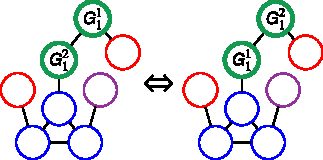
\includegraphics[width=\columnwidth]{../ch2/figures/pisopdf}
\caption{Port-type.\label{fig:ch2:piso}}
\end{subfigure}
\hspace{0.25in}
\begin{subfigure}[b]{2.5in}
\centering
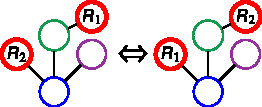
\includegraphics[width=\columnwidth]{../ch2/figures/cisopdf}
\caption{Component-type.\label{fig:ch2:ciso}}
\end{subfigure}
\caption{Two different type of isomorphisms.}
\end{figure}

\item \textit{Component-type isomorphism} occurs when switching a pair of component type  replicates preserves the graph. This type of isomorphism is present due to the arbitrary subscript numbers assigned to each vertex and is demonstrated in Fig.~\ref{fig:ch2:ciso}. The 1-port component type $\xcolor{R}$ is permuted but since $\xcolor{R}_1$ and $\xcolor{R}_2$ are the same component type, the graph remains the same (in the sense of Definition~\ref{def:ch2:ciso}). For $n$ replicates of a component type, there are $n!$ ways to arrange the components such that a component-type isomorphism occurs.

\end{enumerate}
We now define the final graph structure space $\mathcal{G}_3 \subseteq \mathcal{G}_2$ representing all unique useful graphs. Assuming no NSCs except those naturally satisfied by a \mypm{} approach, we can discern a very rough lower bound on the size of this set with:
\begin{align}\label{eq:ch2:lowerbnd}
\mathcal{D}(N_P) \times \prod_{i=1}^{n_C} \frac{1}{R_i! \times (P_i!)^{R_i}} \leq \abs*{\mathcal{G}_3} \leq \mathcal{D}(N_P)
\end{align}

\noindent where this formula assumes all port-type and component-type isomorphisms that could occur, do occur in the set of \mypm{}s. Consider $(C,R,P) = (\xcolor{A},6,1)$, then Eqn.~(\ref{eq:ch2:lowerbnd}) provides a lower bound of 0.02 graphs, but we know there is exactly 1 unique graph.

Although the graph isomorphism problem is NP (nondeterministic polynomial time), there are many efficient practical algorithms \cite{McKay2014a}. Study of the graph isomorphism problem is an ongoing field and recent breakthroughs could lead to improved algorithms \cite{Babai2016a}. In this work, we utilize the python package igraph using the \textsc{isomorphic\_vf2} function \cite{igraph} based on the VF2 algorithm \cite{Cordella2001a} to solve the colored isomorphism problem.

Many architecture design studies ignore the isomorphism problem but presence of isomorphic graphs leads to the evaluation of non-unique options \cite{Schmidt2000a}. For certain problem sizes, the complexity of checking for isomorphisms may be much greater than generating and evaluating new, potentially non-unique graphs. But to understand the effect of problem definition, NSCs, and candidate graph generation algorithms on $\mathcal{G}_3$ requires the isomorphism checks, and can lead to insights into new algorithms that naturally avoid the isomorphism problem \cite{Konigseder2016a}. Other graph generation algorithms have been developed that avoid isomorphic graphs \cite{Read1978a, Faulon2003b}. Furthermore, for appropriately sized problems, the isomorphism check is computationally viable.

% \IncMargin{1em}
\RestyleAlgo{algoruled}

\begin{vAlgorithm}[t]{\columnwidth}{0em}

\LinesNumbered
\SetSideCommentRight 
\DontPrintSemicolon
% \SetNoFillComment

% \SetTitleSty{\textsf}{small}
% \renewcommand{\algorithmcfname}{\small\textbf{\textsf{\MakeUppercase{Algorithm}}}}%

% \SetKwData{Left}{left}\SetKwData{This}{this}\SetKwData{Up}{up}
\SetKwFunction{cumprod}{cumprod}
\SetKwFunction{length}{length}
\SetKwFunction{zeros}{zeros}
\SetKwFunction{ceil}{ceil}
\SetKwFunction{mod}{mod}
\SetKwFunction{mymin}{min}
\SetKwFunction{detectiso}{isomorphic\_vf2}

\SetKwInOut{Input}{Input}
\SetKwInOut{Output}{Output}

\caption{Determination of the unique colored graphs given a set of colored graphs. \label{alg:ch2:cip}}

\Input{$\xvar{Graphs}$ -- set of colored graphs \\
$\xvar{Nbin}$ -- number of bins (for parallel processing)}
\Output{$\xvar{UniqueGraphs}$ -- set of unique colored graphs}
\BlankLine
            
$\xvar{ind}$ $\leftarrow$ $1$ \tcc*{initialize index for total unique graphs}

$\xvar{bin}(1).\xvar{Graphs}(1)$ $\leftarrow$ $\xvar{Graphs}(1)$  \tcc*{first graph is always unique}

	\For(\tcc*[f]{check remaining graphs}){$\xvar{i}\leftarrow$ $2$ \KwTo $\length(\xvar{Graphs})$ }{
	
		$\xvar{G1}$ $\leftarrow$ $\xvar{Graphs}(\xvar{i})$ \tcc*{current graph to check}
		
		\For(\textbf{in parallel} \tcc*[f]{check against each nonempty bin}){$\xvar{j}\leftarrow$ $1$ \KwTo $\mymin(\xvar{Nbin},\xvar{ind})$ }{
		
			$\xvar{k}$ $\leftarrow$ $\length(\xvar{bin(j).Graphs})$ \tcc*{unique graphs in bin}
         
        	$\xvar{IsoFlag}$ $\leftarrow$ $0$ \tcc*{initialize flag, 0 is not isomorphic}
        
        \tcc*[f]{while graphs remain and isomorphism not found}
        
        	\While(){$(\xvar{k} > 0)$ and $(\xvar{IsoFlag} = 0)$ }{
        	
        	$\xvar{G2}$ $\leftarrow$ $\xvar{bin}(\xvar{j}).\xvar{Graphs}(\xvar{k})$ \tcc*{a unique graph}
        
        	\If{\text{$\xvar{G1}$ and $\xvar{G2}$ pass preliminary isomorphism checks}}{
        	
        	$\xvar{IsoFlag}$ $\leftarrow$ $\detectiso(\xvar{G1},\xvar{G2})$ \tcc*{return 1 if G1 and G2 are isomorphic}
        	
        	}
        	        	
        	$\xvar{k}$ $\leftarrow$ $\xvar{k} - 1$ \tcc*{decrease index since G2 checked}
        
        	} % end while loop
        	
			$\xvar{results}(\xvar{j})$ $\leftarrow$ $\xvar{IsoFlag}$ \tcc*{assign result for bin c}
		
		} % end for c
		
		\If(\tcc*[f]{if no isomorphisms}){\text{all elements of  \xvar{results} are $0$} }{
		
        $\xvar{J}$ $\leftarrow$  $\mod(\xvar{ind}, \xvar{Nbin}) + 1$ \tcc*{index for next smallest bin}
        
        $\xvar{bin}(\xvar{J}).\xvar{Graphs}(\xvar{end}+1)$ $\leftarrow$ $\xvar{G1}$  \tcc*{assign to a bin}
        
        $\xvar{ind}$ $\leftarrow$ $\xvar{ind + 1}$ \tcc*{total unique graphs}
        
		
		} % end if statement
		
		
	} % end for i
	
	$\xvar{UniqueGraphs}$ $\leftarrow$  \text{combine graphs in $\xvar{bin}$ into a single set of graphs}

\end{vAlgorithm}

Algorithm~\ref{alg:ch2:cip} was developed to determine $\mathcal{G}_3$ given $\mathcal{G}_2$. This algorithm checks a candidate graph against bins of already found unique graphs and stops checking if an isomorphism is found, making it parallelizable to a degree and removes unnecessary checks. There are a number of quick preliminary checks that can be done between two graphs, as necessary conditions for them to be isomorphic include having the same number of vertices, edges, and color label distributions.